\documentclass[addpoints]{exam}

\usepackage{hyperref}
\usepackage{soul}
\usepackage{tabularx}
\usepackage{tikz}

\usetikzlibrary{positioning}

\graphicspath{{images/}}

% Header and footer.
\pagestyle{headandfoot}
\runningheadrule
\runningfootrule
\runningheader{CS 440}{HW 2: WebGL}{Fall 2021}
\runningfooter{}{Page \thepage\ of \numpages}{}
\firstpageheader{}{}{}

\qformat{{\large\bf \thequestion. \thequestiontitle}\hfill[\totalpoints\ points]}
\boxedpoints

\title{Homework 2: WebGL}
\author{CS 440 Computer Graphics\\Habib University\\Fall 2021}
\date{Due: 2359h on Sunday, 17 October}

\begin{document}
\maketitle

Each problem below specifies the names of the files you have to submit for it. Please make sure your submitted files have the indicated names. Any files in your GitHub repository with these names at the time of the deadline will be considered as your submission.

We will be making use of the utility files from \href{http://interactivecomputergraphics.com/8E/Code\%20update/Common/}{the website} of the newer edition of the textbook. Specifically, we will make use of the files containing ``ES6" in their names. These supersede similarly named files in the folder in that they are compliant with recent JavaScript (JS) standards which deprecate older features which are, in some cases, now considered insecure. You may copy the files \texttt{MVES6.js} and \texttt{initShadersES6.js} to your computer and include the local files in your HTML or include the files over the web as in the \texttt{triangle.html} file in the \textit{Resources} section of Module 5 on the course site on Canvas.

\begin{questions}

  \begin{EnvFullwidth}
    {\Large\bf \hl{Part 1: Getting Up to Speed}}\\
    The problems in this part set up some of the basics required for subsequent parts.
  \end{EnvFullwidth}
  
\titledquestion{Geometry trumps JS}[0]

  We will be using WebGL to render 3D geometry in the browser. Programming for WebGL is done in JS which is not natively aware of geometric types, e.g. vectors. The file, \texttt{MVES6.js} defines abstractions that allow programs to be written in terms of geometric entities, e.g. vector instead of JS array. It also defines a function, \texttt{flatten()}, to convert these types to the required JS types when needed. 

  \underline{Task}: Go over the file {\tt MVES6.js} in order and familiarize yourself with the types that it provides and their related operations. Especially note how the \texttt{mix()} function can be used for interpolating.

  You need not spend too much time understanding the function bodies as long as you can infer, e.g. from the name, what a function does. For now, you may skip the functions in the following sections in the file: ``ModelView Matrix Generators'' and ``Projection Matrix Generators''.

  Wherever possible in your code for subsequent problems, prefer using geometric primitives and operations from {\tt MVES6.js} over native JS types. For this, your HTML file must include the \texttt{MVES6.js} file, either locally or over the web.

\titledquestion{Mapping and Linear Interpolation}[5]
  \label{q:interpolate}

  Linear interpolation between two values and mapping from one range of values to another are common operations in graphics. In this question, we will implement the mapping of a point in one range to another.
  
  \begin{tabularx}{\linewidth}{cX}
    \raisebox{-\totalheight}{
    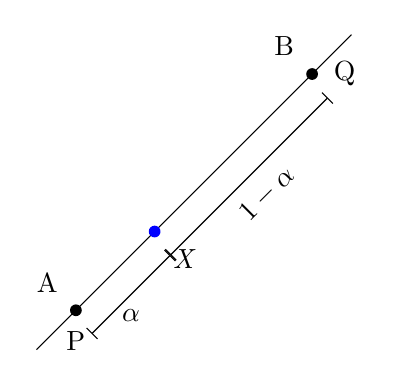
\begin{tikzpicture}
      \draw (0,0) -- (4,4);
      \node[circle,fill,inner sep=1.5pt] at (.5,.5) (P){};
      \node[circle,fill,inner sep=1.5pt] at (3.5,3.5) (Q) {};
      \node[circle,fill,blue,inner sep=1.5pt] at (1.5,1.5) (X) {};
      \node[below  = 2pt of P]{P};
      \node[right = 2pt of Q]{Q};
      \node[below right = 2pt of X]{\it X};
      \node[above left = 2pt of P]{A};
      \node[above left = 2pt of Q]{B};

      \draw[|-|] (0.7,0.2) -- node[midway,below=2pt]{$\alpha$}(1.7,1.2);
      \draw[|-|] (1.7,1.2) -- node[midway,sloped,below=2pt]{$1-\alpha$}(3.7,3.2);
    \end{tikzpicture}
    }
    &
      In the figure on the left, X lies on the line segment PQ such that
      \[
      |PX| : |XQ| = \alpha:(1-\alpha)\;,\; 0 \leq \alpha \leq 1,
      \]
      which leads to
      \[
      X = \alpha Q + (1-\alpha) P.
      \]
      That is, X is an affine combination of P and Q.
      
      Imagine a mapping from the range PQ to a new range AB. For example, P and Q may be vertices and A and B may be the colors assigned to them. We would be interested in finding out the color for X under this mapping. P, Q, and X belong to the same domain. And A and B belong to the same domain. The two domains can be the same, e.g. a mapping of points to points.
  \end{tabularx}

  \underline{Task}: Using \texttt{mix()} from \texttt{MVES6.js}, write a JS function, \texttt{map\_point()}, that takes as argument, P, Q, A, B, and X. P, Q, and X are of the same type. A and B are of the same type. The function returns a value of the same type as A and B and is the mapping of X from the range PQ to the range AB. 

  \noindent\underline{Files}: \texttt{helpers.js}

  \begin{EnvFullwidth}
    {\Large\bf \hl{Part 2: Static Renders}}\\
    We will now begin rendering. finally! The renders in this part are static, i.e. once rendered, they do not change.
  \end{EnvFullwidth}
  
\titledquestion{Maxwell's Triangle}[5]
  \label{q:maxwell}
  
  \begin{tabularx}{\linewidth}{cX}
    \raisebox{-\totalheight}{\includegraphics[width=.35\linewidth]{maxwell}}
    &
      \href{https://en.wikipedia.org/wiki/James_Clerk_Maxwell}{James Clerk Maxwell} is best known for his work in electromagnetic radiation resulting in the well known \href{https://en.wikipedia.org/wiki/Maxwell\%27s_equations}{Maxwell's equations}.
      
      Not surprisingly, he was also among the first ones to explore the \href{https://spie.org/publications/pm105_32_maxwell_triangle?SSO=1}{trichromatic theory of color}. This has led to what is now known as \href{https://homepages.abdn.ac.uk/npmuseum/article/Maxwell/Legacy/MaxTri.html}{Maxwell's triangle}, simply called the \href{https://en.wikipedia.org/wiki/Color_triangle}{color triangle}. It is a triangle with the primary colors at its vertices and its interior shaded by linear combinations of the colors at the vertices. At any interior point, the amount of color contributed by a vertex is proportional to the distance of the vertex from that point.
  \end{tabularx}

  \underline{Task}: WebGL interpolates the colors of the vertices across the primitive by default. Use this property to display Maxwell's triangle: a triangle whose vertices are red, green, and blue.
  
  \underline{Files}: \texttt{maxwell.html, maxwell.js}
  
\titledquestion{The Mandelbrot Set}[15]

  The sequence $z_n$ for a complex number, $c$, is defined for $n\geq 0$ as
  \[
    z_n(c) = \left\{
      \begin{array}{l@{\quad}l}
        0 & n = 0\\
        z^2_{n-1}(c)+c & \textrm{otherwise}
      \end{array}
    \right.
  \]

  \begin{figure}
    \centering
    \begin{tabular}{cc}
      \includegraphics[width=.47\linewidth]{mandelbrot1}& \includegraphics[width=.47\linewidth]{mandelbrot2}\\
      (a) & (b)
    \end{tabular}
    \label{fig:mandelbrot}
    \caption{The Mandelbrot set up to $n_t = 100$. The points at the corners of the windows are outside the circle of radius 2, and $z_n$ escapes for these points at $n=1$. They are completely red. The points in blue toward the center of the image are the ones for which $z_n$ has not yet escaped. (a) Uniform color interpolation from Red to Green to Blue. (b) Adjusted color interpolation on the same data.}
  \end{figure}
  
  The \href{http://en.wikipedia.org/wiki/Mandelbrot_set}{Mandelbrot set}, $M$, is the set of all complex numbers, $c$, for which $z_n(c)$ is \textit{bounded}, i.e. $|z_n|$ is finite for all $n$. It can be shown that if for some $n = n_0$, $|z_{n_0} > 2|$, then the sequence $z_n$ {\it escapes to infinity}, i.e. $|z_n|$ is not bounded for $n > n_0$. This leads to the conclusion that $\forall c \in M:\, z_n(c) \leq 2$. Since $z_1 = c$, the above condition also implies that $|c| \leq 2$.
  The above yields the following two handy conditions whose fulfillment by a complex number, $c$, establishes its membership in $M$:
  \begin{enumerate}
  \item $|c|\leq 2$
  \item $\forall n\geq 0:\, |z_n(c)|\leq 2$
  \end{enumerate}
  The value of $n$ for which condition 2 becomes false for a given $c$ is dubbed the {\it escape time} of $c$. Condition 2 also implies that all members of the Mandelbrot set lie within the circle in complex plane centered at the origin and with radius 2.

  \underline{Example}: Consider the following complex numbers and the corresponding sequence for each up to $z_5$.
  \[
    \begin{array}{c|*{4}{|c}}
      & c=(3+4j) & c=(1+1j) & c=(0.5+0.5j) & c=(-0.5-0.5j)\\\hline\hline
      z_0(c) & 0 & 0 & 0 & 0\\
      |z_0(c)| & 0 & 0 & 0 & 0\\\hline
      z_1(c) & (3+4j) & (1+1j) & (0.5+0.5j) & (-0.5-0.5j)\\
      |z_1(c)| & 5.0 & 1.41 & 0.71 & 0.71\\\hline
      z_2(c) &  & (1+3j) & (0.5+1j) & (-0.5+0j)\\
      |z_2(c)| &  & 3.16 & 1.12 & 0.5\\\hline
      z_3(c) &  &  & (-0.25+1.5j) & (-0.25-0.5j)\\
      |z_3(c)| &  &  & 1.52 & 0.56\\\hline
      z_4(c) &  &  & (-1.69-0.25j) & (-0.69-0.25j)\\
      |z_4(c)| &  &  & 1.71 & 0.73\\\hline
      z_5(c) &  &  & (3.29+1.34j) & (-0.09-0.16j)\\
      |z_5(c)| &  &  & 3.55 & 0.18\\\hline
    \end{array}
  \]

  \begin{itemize}
  \item We see that $z_1=c$. This follows from the definition of $z_n$.
  \item For the first number, $(3+4j)$, we see that $|z_1|>2$. We can therefore say that $z_n$ will escape to infinity and the escape time of $(3+4j)$ is 1. This expected as $(3+4j)$ lies outside the circle at the origin with radius 2.
  \item The second number, $(1+1j)$, lies within the required circle. But it escapes at n=2.
  \item The escape time for the third number, which is also inside the circle, is 5.
  \item The fourth number in also inside the circle and has not escaped until n=5. It may escape later or it may not. We cannot say.
  \end{itemize}
  
  \underline{Problem}: We want to visualize the Mandelbrot set up to a certain value of $n=n_t$ in an image. We will map to our viewport the circle in the complex plane which is centered at the origin and has a radius of 2. This will yield the complex number corresponding to each pixel in the view port. We will color each pixel according to the escape timeof its corresponding complex number. In Figure \ref{fig:mandelbrot}, complex numbers that escape early are assigned red and those that have not escaped till $n=n_t$ are assigned blue. Complex numbers with intermediate escape values are assigned interpolated colors. 

  Various steps are involved.
  \begin{enumerate}
  \item Map the x extent of our image to $[-2,2]$ on the real axis in the complex plane.
  \item Map the y extent of our image to $[-2j,2j]$ on the imaginary axis in the complex plane.
  \item Find the escape time of the complex number corresponding to each pixel in the image,
  \item Compute a color for a given escape time.
  \end{enumerate}

  \underline{Task}: Visualize the Mandelbrot set as described above with $n_t$ defined as a global variable at the beginning of your JS file. You will find that a simple linear interpolation between the colors for $n=1$ and $n=n_t$ will lead to a bland visualization as seen in Figure \ref{fig:mandelbrot}a). You are encouraged to think about and implement an appropriate coloring scheme for the escape times. You may implement any coloring scheme that sufficiently distinguishes between different escape times.

  \underline{Tips and Notes}:\\
  --\ As you may imagine, this computation can be expensive. Pick an $n_t$ that is feasible for your machine and leads to an interesting visualization.\\
  --\ Make liberal use of the \texttt{map\_point()} function. Points 1, 2, and 4 above lend themselves simply to its use.\\
  --\ You are encouraged to use the \texttt{Complex} type from \texttt{math.js}. See its usage \href{https://mathjs.org/docs/datatypes/complex_numbers.html}{here}. To use it in your JS code, include the following line in your HTML file.\\
  \centerline{\texttt{<script src="https://unpkg.com/mathjs@9.5.0/lib/browser/math.js"></script>}}

  \noindent\underline{Files}: \texttt{mandelbrot-cpu.html, mandelbrot-cpu.js}

\titledquestion{Mandelbrot meets GPU}[15]
  The main task in visualizing the Mandelbrot set is to determine the color at each pixel. The calculation at each pixel is completely independent of the other pixels. This task is perfectly suited for the fragment shader, whose sole task is to compute the color of the pixel. In this question, we will render the same visualization as above but perform the related computation on the GPU.

  \underline{Task}: Visualize the Mandelbrot set as described in the previous question by performing the color related computation in the fragment shader. There are several issues to tackle here.
  \begin{itemize}
  \item What data needs to be passed to the fragment shader: what information does the fragment shader need in order to compute the color.
  \item What data needs to be passed to the vertex shader: our program does not talk to the fragment shader, rather it can pass data to the vertex shader which can then pass data to the fragment shader.
  \item What attributes need to be passed to the vertex shader: the vertex shader runs once per vertex but vertices define a polygon which rasterizes to numerous pixels and the fragment shader runs for each pixel. The attributes passed to the vertex shader must be such that each rasterized pixel obtains a version of the data that is right for it.
  \item Writing complex number arithmetic: GLSL does not natively support complex numbers. You will have to define functions in your shader to work with complex numbers.
  \item Many others.
  \end{itemize}
  Thinking about and finding solutions to these sub-problems is an intended part of this problem.

  \underline{Tips and Notes}:
  \begin{itemize}
  \item Make sure that you conceptually understand the problem and the solution before you open your code editor.
  \item GLSL has some helpful syntax and types to support geometric computation. You can read about it in the GLSL section toward the bottom of \href{https://webgl2fundamentals.org/webgl/lessons/webgl-shaders-and-glsl.html}{this page}.
  \end{itemize}
  
  \noindent\underline{Files}: \texttt{mandelbrot-gpu.html, mandelbrot-gpu.js}
  
  \begin{EnvFullwidth}
    {\Large\bf \hl{Part 3: Interactive Rendering}}\\
    Rendering is cool. More so when it responds to user input. The renders in this part are dynamic and interactive. They update based on the user's interaction with interactive widgets on the page.
  \end{EnvFullwidth}
  
\titledquestion{Tetrix}[15]

  \begin{tabular}{ccc}
    \includegraphics[width=.3\textwidth]{tetrix1}
    & \includegraphics[width=.3\textwidth]{tetrix2}
    & \includegraphics[width=.3\textwidth]{tetrix3}
  \end{tabular}
  In this question, we will interactively render a \href{http://mathworld.wolfram.com/Tetrix.html}{\it tetrix} which is the 3D version of the Sierpinski triangle and is also referred to as the \textit{Sierpinski tetrahedron}. By default the tetrix will continuously rotate about an arbitrary axis of your choice. Interactive controls will let the user toggle rotation, reset the tetrix to a default position, and change the axis of rotation. An interactive slider specifies the recursion level of the tetrix. A recursion level of 0 corresponds to a completely filled tetrahedron. The left-most tetrix in the figure corresponds to a recursion level of 1.

  \underline{Task}: Visualize the tetrix as described above. The interactive elements, e.g. the slider for the recursion level, should take effect immediately. The slider should be bounded between reasonable values.

  \noindent\underline{Files}: {\tt tetrix.html, tetrix.js}

\titledquestion{Polygons Galore}[15]
  \label{q:galore}
  
  \begin{tabularx}{\linewidth}{lX}
    \raisebox{-.9\totalheight}{\includegraphics[width=.35\textwidth]{galore}}
    &
      We love polygons and cannot get enough of them. For this problem, we will make a program to draw a limited set of polygons. The user will specify vertices through mouse clicks and once the right number of vertices have been specified, the program will connect them into a polygon determined by the current drawing mode. For example, if \textit{triangle mode} is on, every 3 successive vertices will be connected to form a triangle.
  \end{tabularx}
  \underline{Task}: Write a program that interactively draws triangles and quadrilaterals based on vertices specified by mouse clicks in the canvas. The program supports two {\it modes}--triangle mode (default) and quad mode. Vertices that are not yet part of a polygon are drawn as points. Each drawn shape is assigned a different random color. Furthermore, the following interaction is supported.
  \begin{parts}
  \part Pressing \texttt{r} or \texttt{R} resets to default. That is, the canvas is cleared and the drawing mode is set to triangle mode.
  \part Pressing \texttt{t} or \texttt{T} toggles between the drawing modes. Vertices that have not yet completed a polygon at the time of the toggle should be handled according to the new mode, they should not be discarded. Polygons drawn before the toggle should not be affected.
  \end{parts}
  \noindent\underline{Files}: {\tt galore.html, galore.js}

\titledquestion{Reflex Game}[20]

  Sitting in front of the computer, staring passively at the screen is making us all dull. You decide to help people use their screen time productively by making a game that will sharpen their reflexes. In the game, the player has to click on a polygon that appears for a brief period at a random location on screen. After a fixed interval the polygon disappears and reappears at another random location. If the player is able to click inside the polygon before it disappears, her score increments and the polygon disappears to reappear at another location. If she clicks on a blank location, e.g. the polygon there has already disappeared, her score decrements. If she has not clicked at all for three consecutive polygons, her score decrements. The player starts the game with a score of 0 and the game ends when her score becomes negative.

  \underline{Task}: Write the above game. All rendering and interaction takes place inside the canvas. Make sure that at most 1 polygon is drawn on the canvas at any given time.
  
  \underline{Files}: {\tt reflex.html, reflex.js}

  \begin{EnvFullwidth}
    {\Large\bf \hl{Part 4: I wanna fly}}\\
    This part contains suggestions to add more punch to your renders. These are just suggestions, you may implement others. For the benefit of your reviewer, make sure to prominently mention any additional functionality on the HTML page. Also, make sure to commit the basic version of your render so that you can always roll back to it in case the embellishments do not quite work out.

    These are for your intellectual and aesthetic satisfaction and for the enjoyment of your peer reviewer. Such benefits and outcomes are self-rewarding and transcend quantification. We will not commit the barbarity of assigning marks to them.

    Viel Spa\ss!
  \end{EnvFullwidth}

\titledquestion{Superpowers}[0]

  Here are some suggestions to make your renders even cooler. Feel free to implement others.

  \textbf{Tetrix}: Color the faces of the tetrahedra according to some scheme.
  
  \textbf{Mandelbrot}: Let the user control $n_t$ through an interactive slider and update the visualization accordingly in real time. This applies to the GPU version which is faster and should be more responsive.
  
  \textbf{Galore}: Implement additional polygon modes.
  
  \textbf{Reflex}: Quite a few suggestions:
  \begin{parts}
  \part Appearance: the shape and color of the polygon change between appearances.
  \part Score: the current score is displayed and updated on the page.
  \part Game speed: the duration of the polygon's appearance on screen is adaptive. It decreases as the player's score increases and increases if the player loses score due to wrong clicks or lack of clicks.
  \part Time: a timer appears on the page that counts down from 30 seconds. The game ends as before or when the timer reaches 0.
  \end{parts}

\end{questions}

\end{document}
%%% Local Variables:
%%% mode: latex
%%% TeX-master: t
%%% End:
